\documentclass[aspectratio=169]{beamer}

\usepackage{tikzlings}
\usetikzlibrary{decorations.text,fpu}

\setbeamertemplate{navigation symbols}{}

% trick taken from https://topanswers.xyz/tex?q=1989
\tikzset{
    use page relative coordinates/.style={
        shift={(current page.south west)},
        x={(current page.south east)},
        y={(current page.north west)}
    },
}

\makeatletter
\newcommand*{\slideinframe}{\number\beamer@slideinframe}
\makeatother

\begin{document}

\def\steps{700}
\begin{frame}
  \begin{tikzpicture}[
      remember picture,
      overlay
    ]
    
    \begin{scope}[use page relative coordinates]
      \node[anchor=north,inner sep=0pt] at (current page.north) {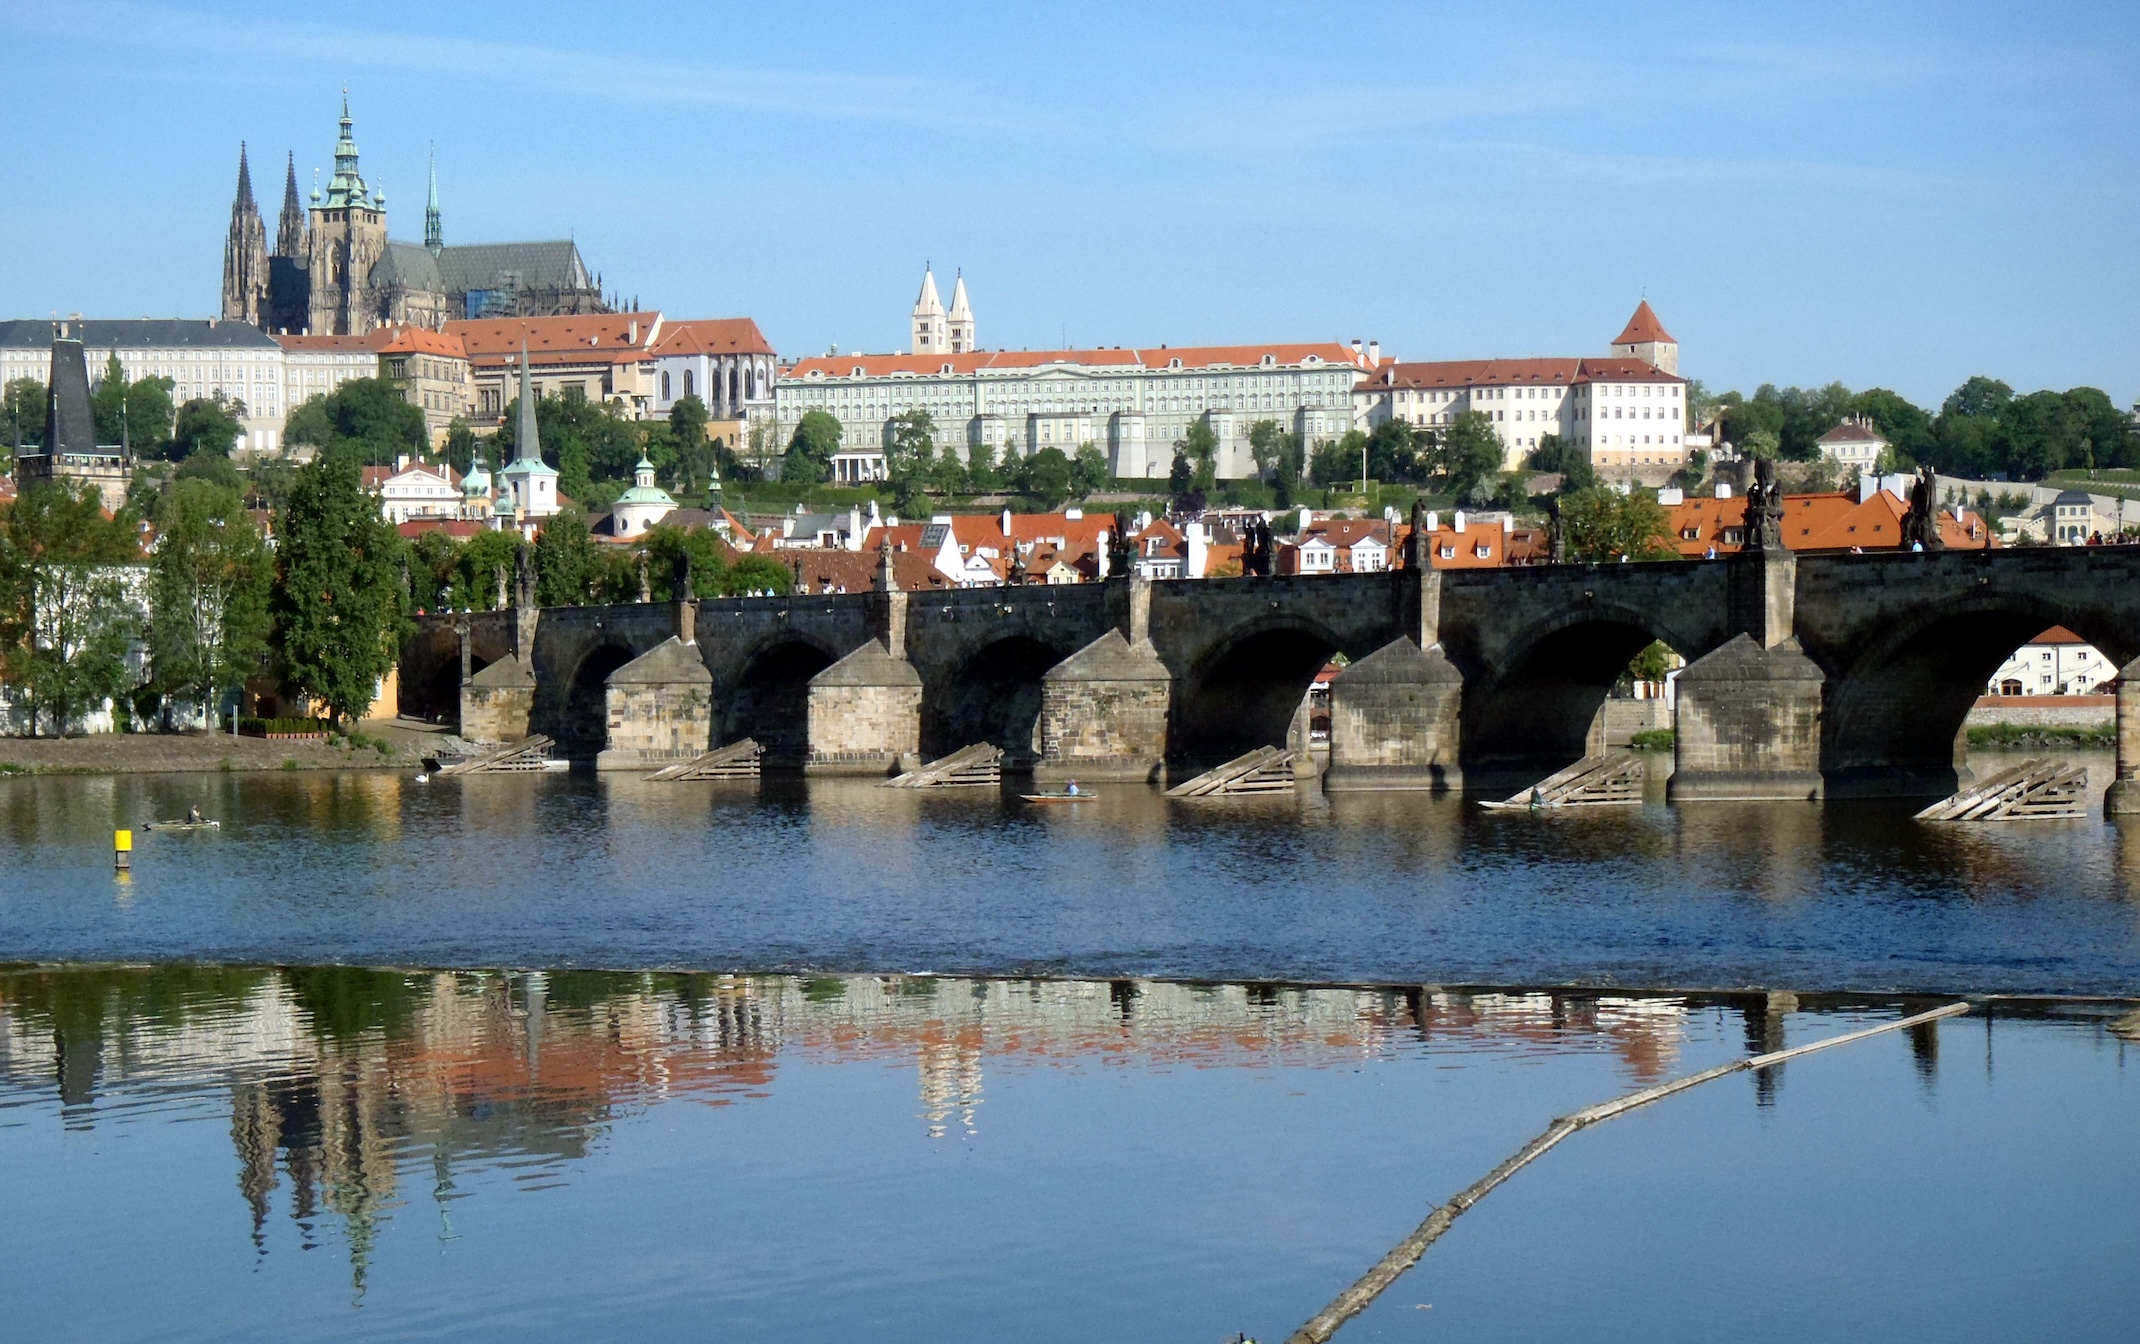
\includegraphics[width=\paperwidth]{Charles_bridge_and_Prazsky_Hrad_-_panoramio}};
        
      \node at (-0.5+1.5*\slideinframe/\steps,0.15+0.29*\slideinframe/\steps) {
\includegraphics[height=1cm]{clip_duck}};

      \node[anchor=north,inner sep=0pt] at (current page.north) {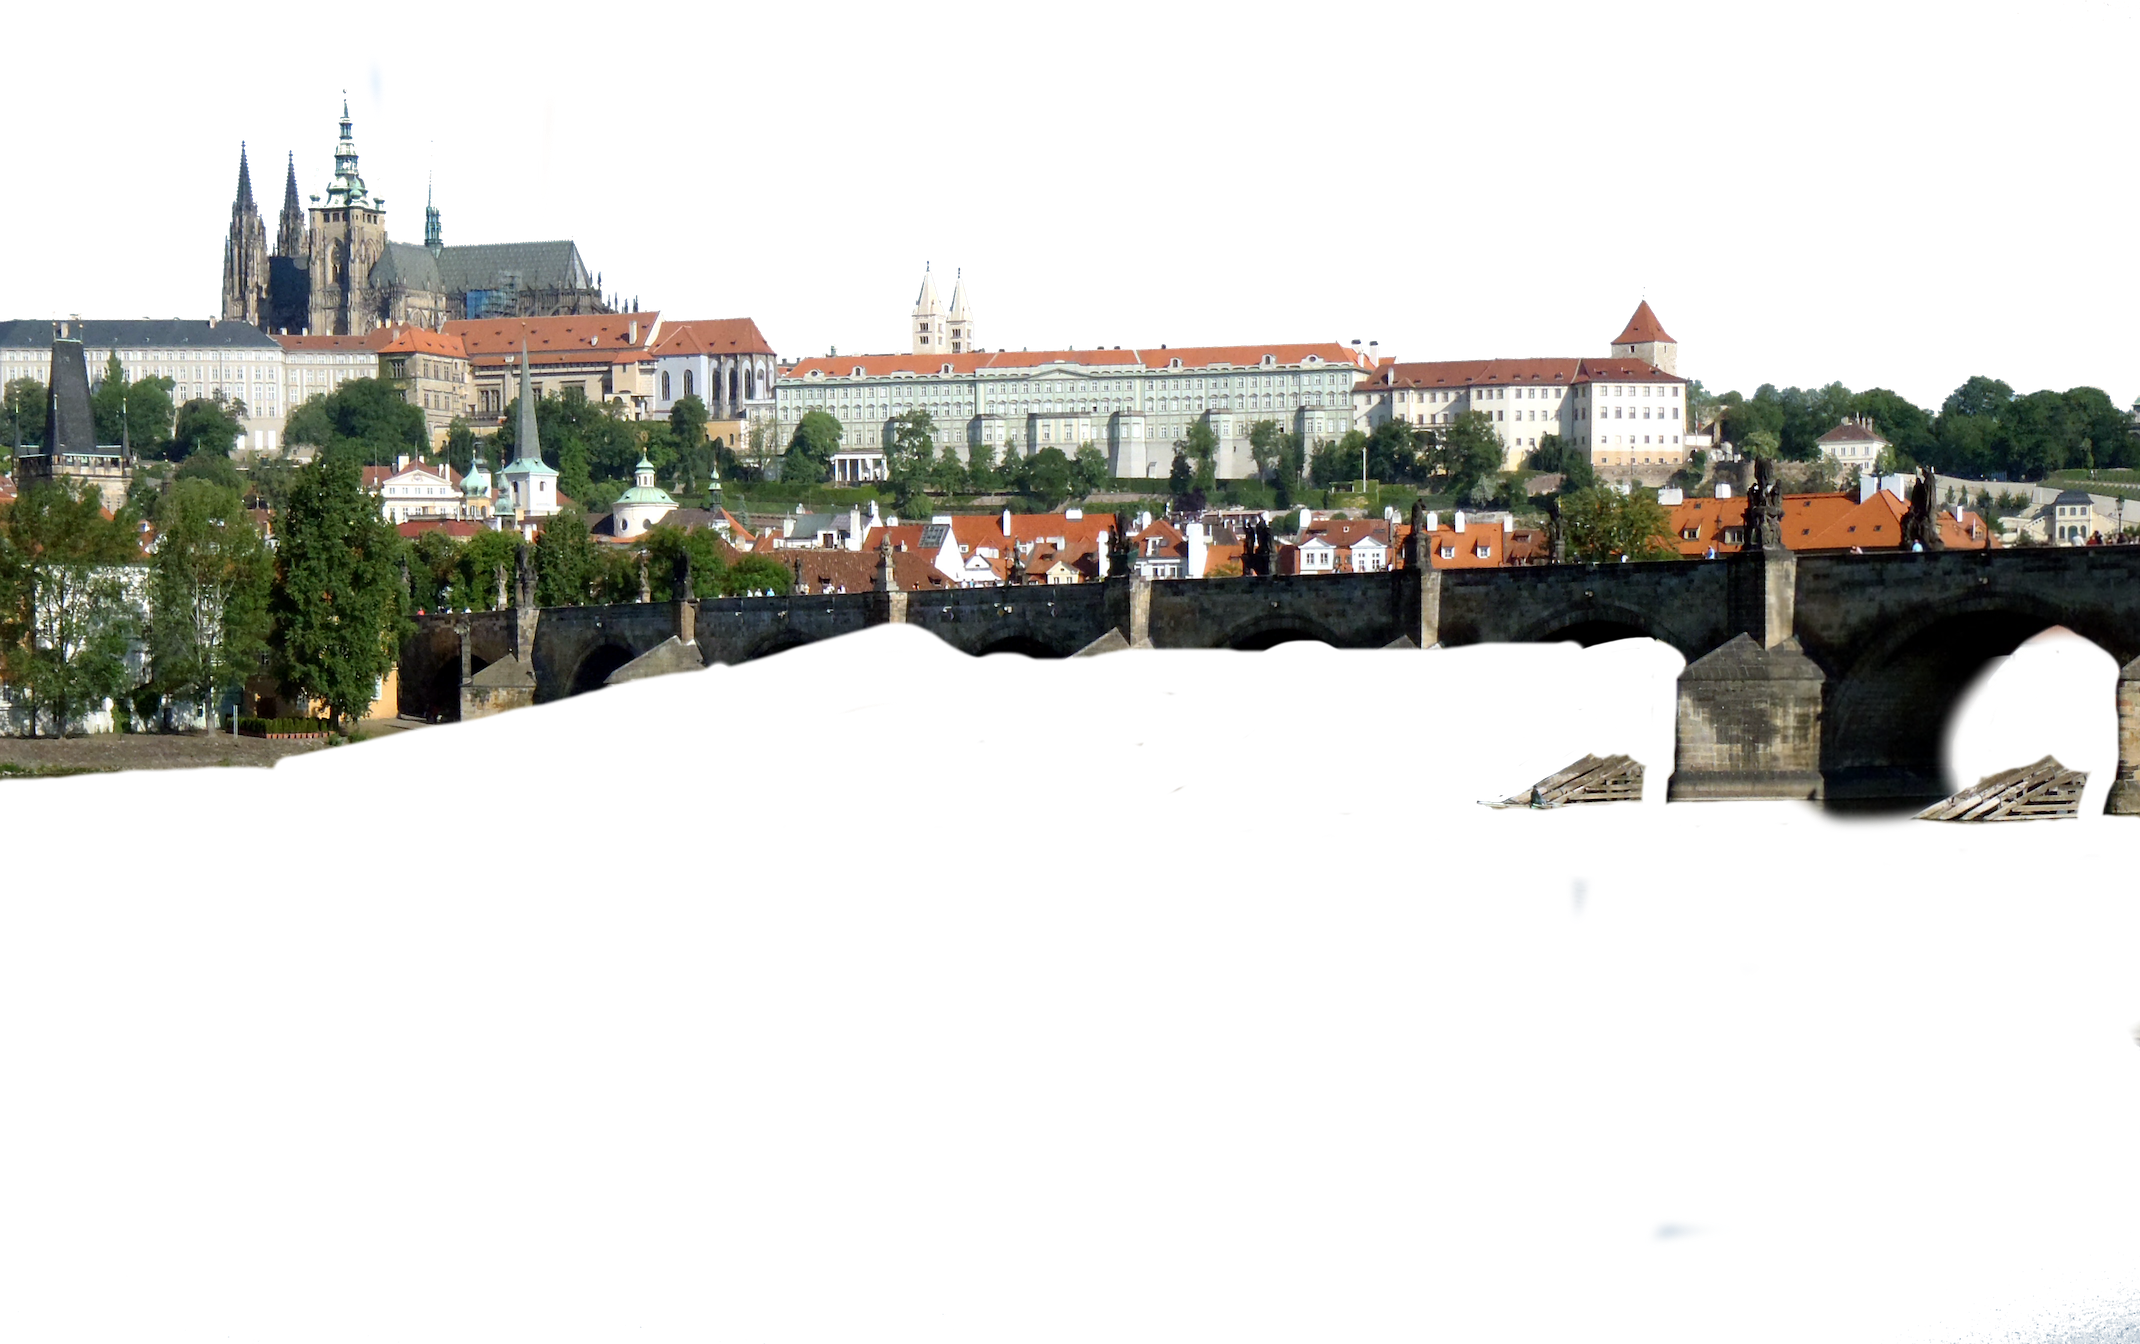
\includegraphics[width=\paperwidth]{Charles_bridge_and_Prazsky_Hrad_-_panoramio_fg}};
     
      \node at (-1.5+2*\slideinframe/\steps,-0.5+0.83*\slideinframe/\steps) {
\includegraphics[height=1cm]{clip_duck}};            
      
      \node at (-0.1+1*\slideinframe/\steps,-0.1+0.42*\slideinframe/\steps) {
\includegraphics[height=1cm]{clip_duck}};    
  
      % credit for background image
      \node[white,text width=\paperwidth,font=\tiny,align=center] at ([yshift=0.25cm]current page.south) {Image by Eric Spenle (\url{https://commons.wikimedia.org/wiki/File:Charles_bridge_and_Prazsky_Hrad_-_panoramio.jpg})};        
    \end{scope}
    
    \begin{scope}[remember picture,overlay,transform canvas={scale=0.5}]
      \pgfmathparse{35-\slideinframe/\steps*45}
      \begin{scope}[xshift=\pgfmathresult cm,yshift=5cm]
        \pgfmathparse{cos(3*\slideinframe)*1.5}
        \coordinate (a) at (0,0);
        \coordinate (b) at (2.7,\pgfmathresult);
        \coordinate (c) at (5.4,-\pgfmathresult);
        \coordinate (d) at (8,0);
        \draw[thick] ([yshift=1cm]a) -- (-2,0.3) -- ([yshift=-0.4cm]a) -- cycle;
        \node at (-2,0.3) {
\includegraphics[width=3cm]{AirDuck}};
        \fill[white!90!black,draw=black,thick] ([yshift=-0.4cm]a) .. controls ([yshift=-0.4cm]b) and ([yshift=-0.4cm]c) .. ([yshift=-0.4cm]d) -- ([yshift=1cm]d) .. controls ([yshift=1cm]c) and ([yshift=1cm]b) .. ([yshift=1cm]a) -- ([yshift=-0.4cm]a) ;
        \path [
          decorate,
          decoration={text along path,pre length=0.5cm,text={|\Huge\bfseries|TUG'24 @ Prague}}
        ] (a) .. controls (b) and (c) .. (d);
      \end{scope}
    \end{scope}  
  \end{tikzpicture}  
  \pause[\steps]
\end{frame}

\end{document}